% --------------------------------------------------------------
% Abhi's Standard math Preamble.
% --------------------------------------------------------------
 
% Document packages / layout
\documentclass[
    pdf,
    10pt,
    xcolor={svgnames},
    %hyperref={colorlinks, citecolor=Cyan, linkcolor=Cyan, urlcolor=Cyan}
  ]{beamer}
%\usetheme{Copenhagen}
\usetheme{Madrid}
\usecolortheme{beaver}
\usepackage{color}
\setbeamertemplate{navigation symbols}{}%remove navigation symbols

\newcommand\hmmax{0}
\newcommand\bmmax{0}

\usepackage{biblatex}
\addbibresource{citations.bib}

\newcommand\blfootnote[1]{%
  \begingroup
  \renewcommand\thefootnote{}\footnote{#1}%
  \addtocounter{footnote}{-1}%
  \endgroup
}

% Figure Packages
\usepackage{float}
\usepackage{subcaption}

% Math Packages
\usepackage{amsmath, amsthm, amssymb}
\usepackage{commath} %for \norm and \abs
\usepackage{bm}
\usepackage{dsfont}
\usepackage{mathtools}
\usepackage{mathrsfs}
\usepackage{physics}
\usepackage{stmaryrd}
\allowdisplaybreaks

% Quality of Life Packages
\usepackage{enumerate}
\usepackage{siunitx} %\sisetup{inter-unit-product =$\cdot$}
\usepackage{multicol}

\newtheorem*{lemma*}{Lemma}
\newtheorem*{theorem*}{Theorem}

%% general package aliases
\newcommand{\bs}{\boldsymbol}
\def\ds{\displaystyle}
\newcommand{\mb}[1]{\mathbb{#1}}
\newcommand{\mc}[1]{\mathcal{#1}}
\newcommand{\ms}[1]{\mathscr{#1}}
%% Set aliases
\newcommand{\N}{\mathbb{N}}
\newcommand{\R}{\mathbb{R}}
%% Analysis aliases
\newcommand{\e}{\varepsilon}
\DeclareMathOperator*{\argmin}{\arg\!\min}
\DeclareMathOperator*{\argmax}{\arg\!\max}
\DeclarePairedDelimiterX{\inp}[2]{\langle}{\rangle}{#1, #2}
%% Matrix aliases
\newcommand{\T}{\mathrm{T}}
\renewcommand{\vec}[1]{{\mathchoice
                     {\mbox{\boldmath$\displaystyle{#1}$}}
                     {\mbox{\boldmath$\textstyle{#1}$}}
                     {\mbox{\boldmath$\scriptstyle{#1}$}}
                     {\mbox{\boldmath$\scriptscriptstyle{#1}$}}}}
\newcommand{\mat}[1]{\mathbf{{#1}}}
%% Inverse Problems aliases
\newcommand{\Reg}{\boldsymbol{\mathcal{R}}}
\newcommand{\priormean}{\vec{u}_{0,{\rm pr}}}
\newcommand{\ut}[1]{\ensuremath{\tilde{#1}}}
\newcommand{\ui}[1]{\ensuremath{\hat{#1}}}
\newcommand{\bui}[1]{\ensuremath{\hat{\boldsymbol{#1}}}}
\newcommand{\bu}[1]{\ensuremath{\boldsymbol{#1}}}
\newcommand{\mbu}[1]{\ensuremath{\mathbf{#1}}}
\newcommand{\obs}{\mathbf{u}^{\rm obs}}

% Creates section subdivider at beginning of each section.
\AtBeginSection[]
{
  \begin{frame}
    \frametitle{Table of Contents}
    \tableofcontents[currentsection]
  \end{frame}
}
 
\title[%
  Fault slip inversion via Bayesian inference
]{%
  Infinite-dimensional Bayesian inversion for fault slip from surface measurements
}
\author[Chowdhary, Alexanderian]{%
  Abhijit Chowdhary and Alen Alexanderian
}
\institute[NCSU]{
  Department of Mathematics \\
  North Carolina State University
}
\date[AMGSS 2022]{\today}

\begin{document}
 
\frame{ \titlepage \scriptsize{ Work done through NSF-DMS-2111044 } }

\begin{frame}
  \begin{figure}
    \centering
    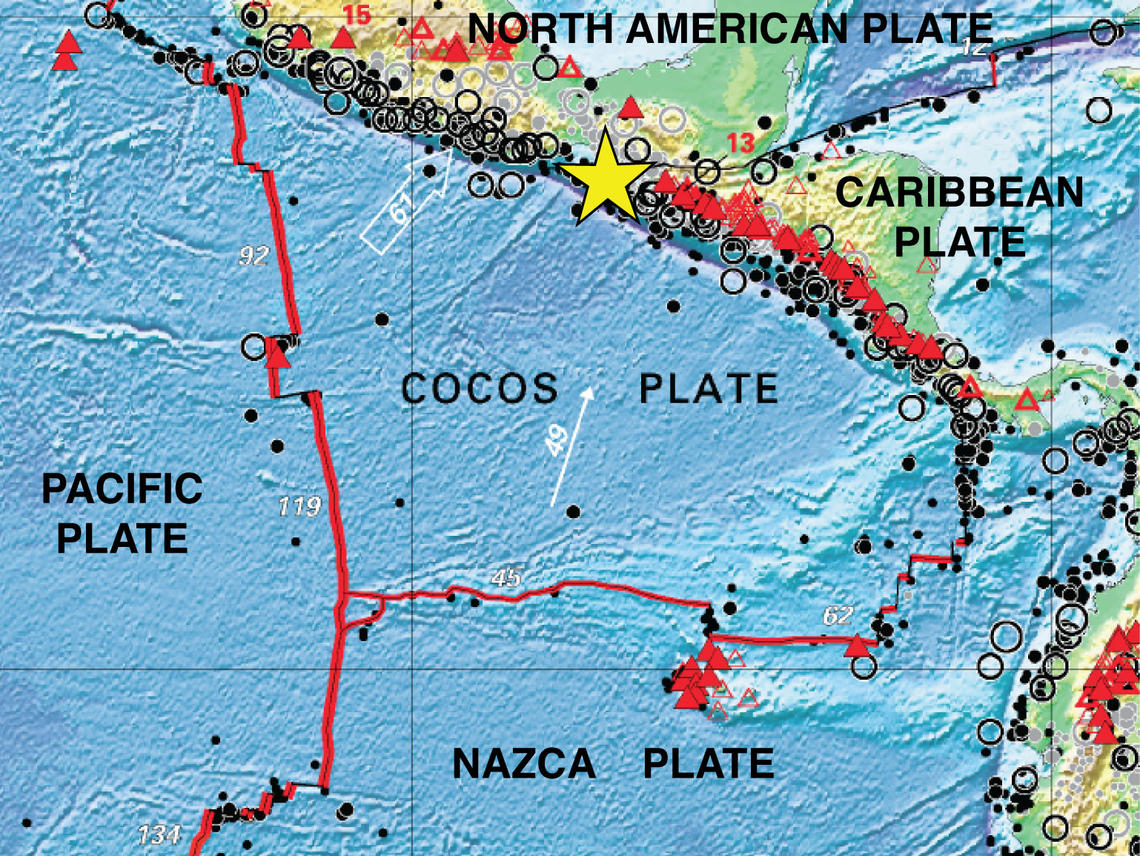
\includegraphics[width=0.85\textwidth]{./resources/Cocos}
  \end{figure}
  \blfootnote{\fullcite{Cocos2006}}
\end{frame}

\begin{frame}
  \begin{figure}
    \centering
    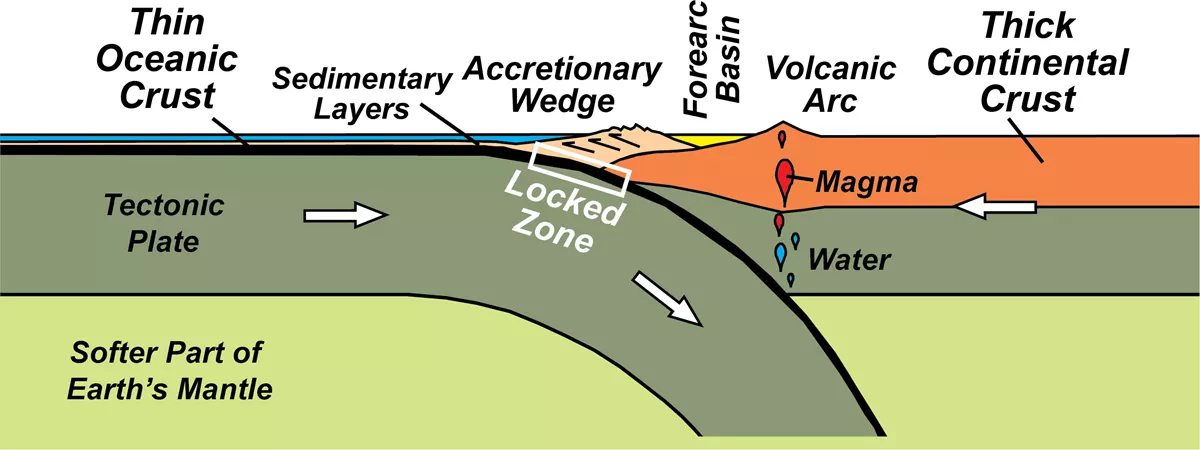
\includegraphics[width=\textwidth]{./resources/subduction_zone}
  \end{figure}
  \blfootnote{\fullcite{Lillie2017}}
\end{frame}

\begin{frame}
  \frametitle{Goals}
  \begin{alertblock}{}
    \begin{center}
      {\large Understand the subduction zone from collected observations.}
    \end{center}
  \end{alertblock}
  \pause
  \begin{alertblock}{}
    \begin{center}
      {\large Do so while quantifying measurement uncertainties.}
    \end{center}
  \end{alertblock}
\end{frame}

\begin{frame}
  \frametitle{Table of Contents}
  \tableofcontents
\end{frame}

%%%%%%%%%%%%%%%%%%%%%%%%%%%%%%%%%%%%%%%%%%%%%%%%%%%%%%%%%%%%%%%%%%%%%%%%%%%%%%%
%%% Seismic Inversion Model Problem
%%%%%%%%%%%%%%%%%%%%%%%%%%%%%%%%%%%%%%%%%%%%%%%%%%%%%%%%%%%%%%%%%%%%%%%%%%%%%%%
\section{Seismic Inversion Model Problem}
\begin{frame}
  \frametitle{Model Assumptions}
  \begin{figure}
    \centering
    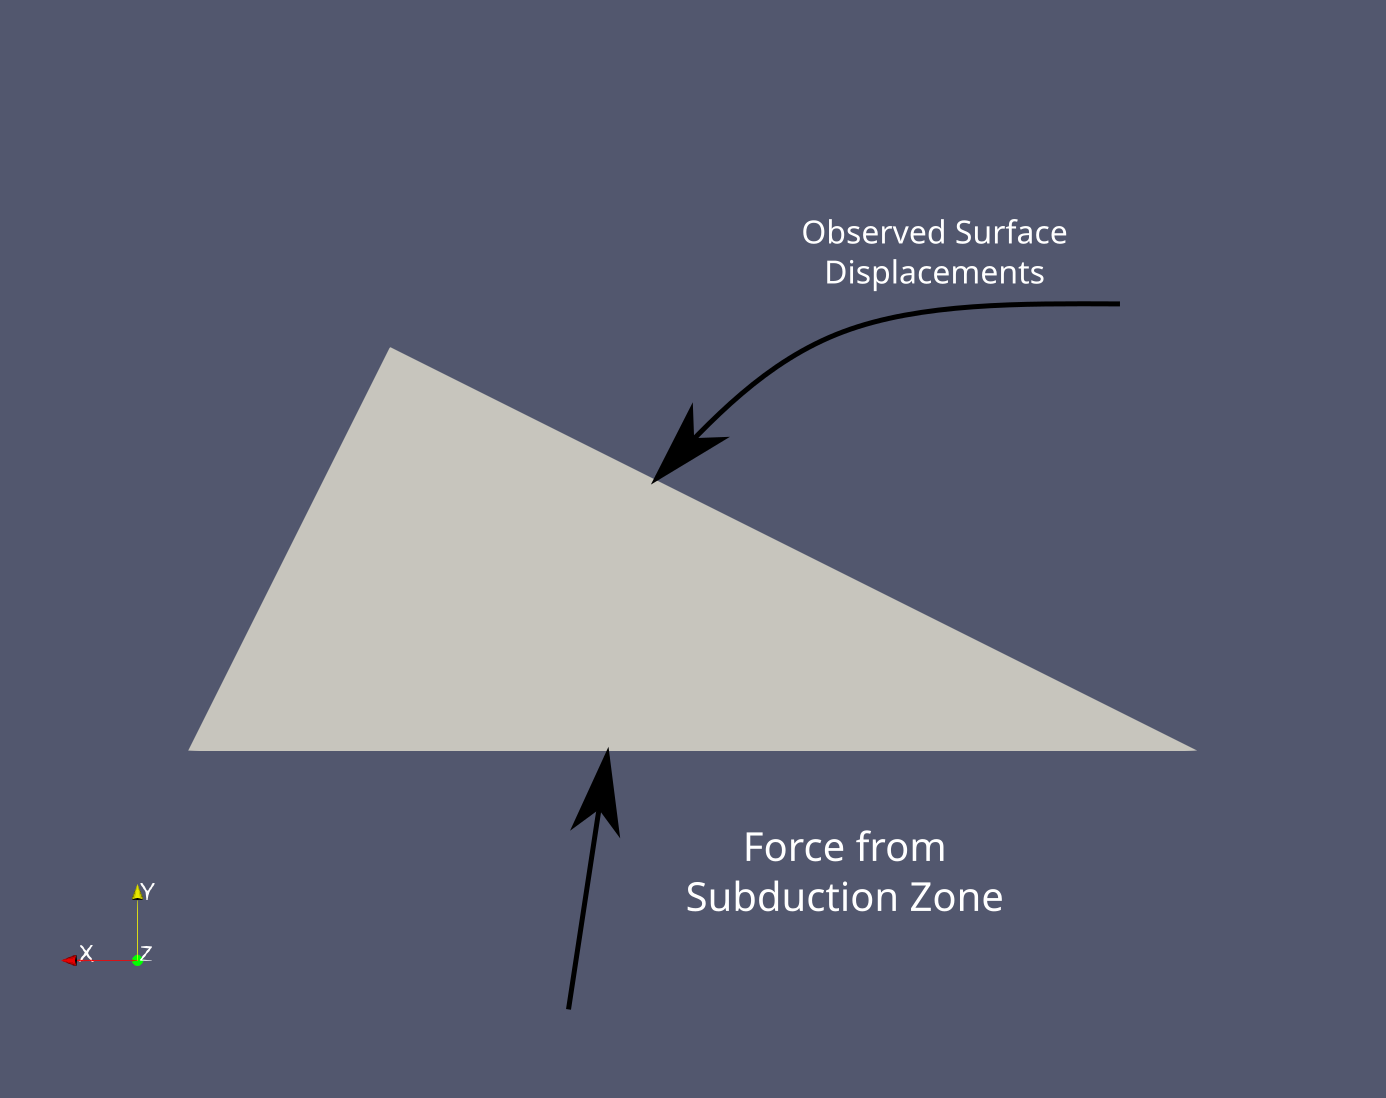
\includegraphics[width=0.55\textwidth]{./resources/triangle_paraview}
    %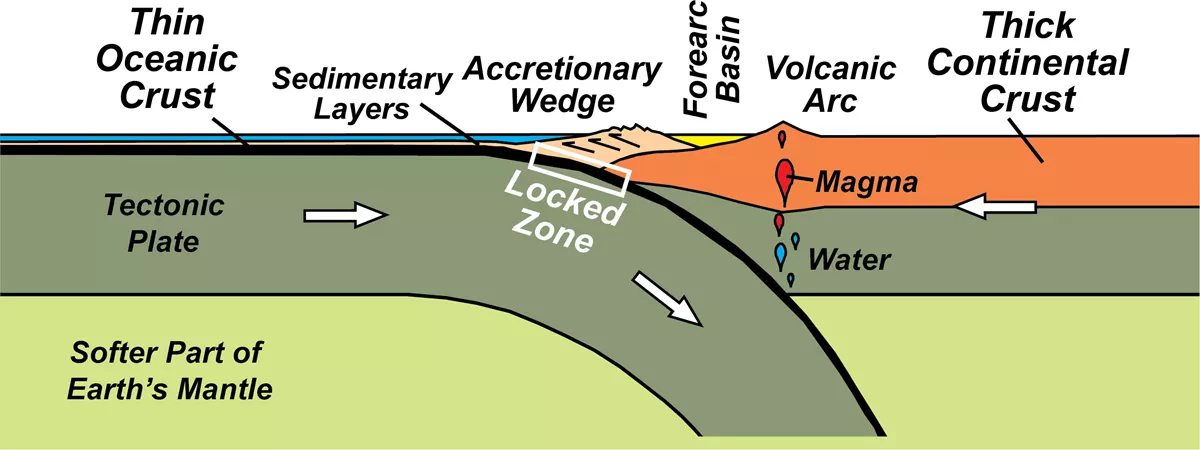
\includegraphics[width=\textwidth]{./resources/subduction_zone}
  \end{figure}
  For the sake of modeling convienience, assume:
  \begin{itemize}[<+->]
    \item \textbf{Governing PDE} (forward model): Linear elasticity
    \item \textbf{Uncertain parameter}: Displacement on fault plane
    \item \textbf{Inverse Problem}: Given measurements of surface deformation
      $\obs$ reconstruct fault plane displacement.
  \end{itemize}
\end{frame}
\begin{frame}
  \frametitle{Forward Model}
  \begin{equation}
    -\nabla \cdot \bs \sigma(\bs u) = \bs 0 \text{ in } \Omega,
  \end{equation}
  where:
  \begin{itemize}
    \item $\vec{\sigma}(\vec{u}) = \mathbb{C} \vec{\varepsilon}(\vec{u})$ with 
    \begin{itemize}
      \item $\mathbb{C}[\vec{\e}] = 2\mu \vec{\e} + \lambda \tr(\vec{\e})
        \mat{I}$ the fourth-order linear elasticity tensor:
      \item $\vec{\e}(\vec{u}) = \frac{1}{2} \left[ \grad \vec{u} + (\grad
        \vec{u})^\T \right]$ the strain tensor.
    \end{itemize}
  \item $\mu$ and $\lambda$ are known as the L\'{a}me constants.
  \end{itemize}
  \blfootnote{\fullcite{McCormack2018}}
\end{frame}
\begin{frame}
  \frametitle{Forward Model}
  \begin{subequations}\label{eq:elast_strong}
    \begin{align}
      - \grad \left[ 
        \mu(\grad \vec{u} + (\grad \vec{u})^\T)
        + \lambda \div \vec{u} \mat{I}
      \right]
      &=
      \label{eq:elast_strong_a}
      \vec{0} \quad \text{in } \Omega, \\
      \label{eq:elast_strong_b}
      \vec{\sigma}(\vec{u}) \vec{n} 
      &= 
      \vec{0} \quad \text{on } \Gamma_t \\
      \label{eq:elast_strong_c}
      \vec{u} + \beta \vec{\sigma}(\vec{u}) \vec{n}
      &=
      \vec{h} \quad \text{on } \Gamma_s \\
      \label{eq:elast_strong_d}
      \vec{u} \vdot \vec{n} 
      &=
      0 \quad \text{on } \Gamma_b \\
      \label{eq:elast_strong_e}
      \delta \mat{T}(\vec{\sigma}(\vec{u})\vec{n}) + \mat{T}\vec{u}
      &=
      \vec{m} \quad \text{on } \Gamma_b
    \end{align}
  \end{subequations}
  \begin{itemize}[<+->]
    \item $\mat{T}$ is the tangential operator $\mat{T} \vec{u} = (\mat{I}
      - \vec{n} \otimes \vec{n}) \vec{u} = \vec{u} - (\vec{n}^\T \vec{u})
      \vec{n}$.
    \item The right hand side of \eqref{eq:elast_strong_e} is the displacement
      on the fault plane that is being inverted for.
    \item \eqref{eq:elast_strong_e} can be understood as a regularized Dirichlet
      condition.
  \end{itemize}
\end{frame}

\begin{frame}
  \frametitle{Forward Solution}
  \begin{figure}
    \centering
    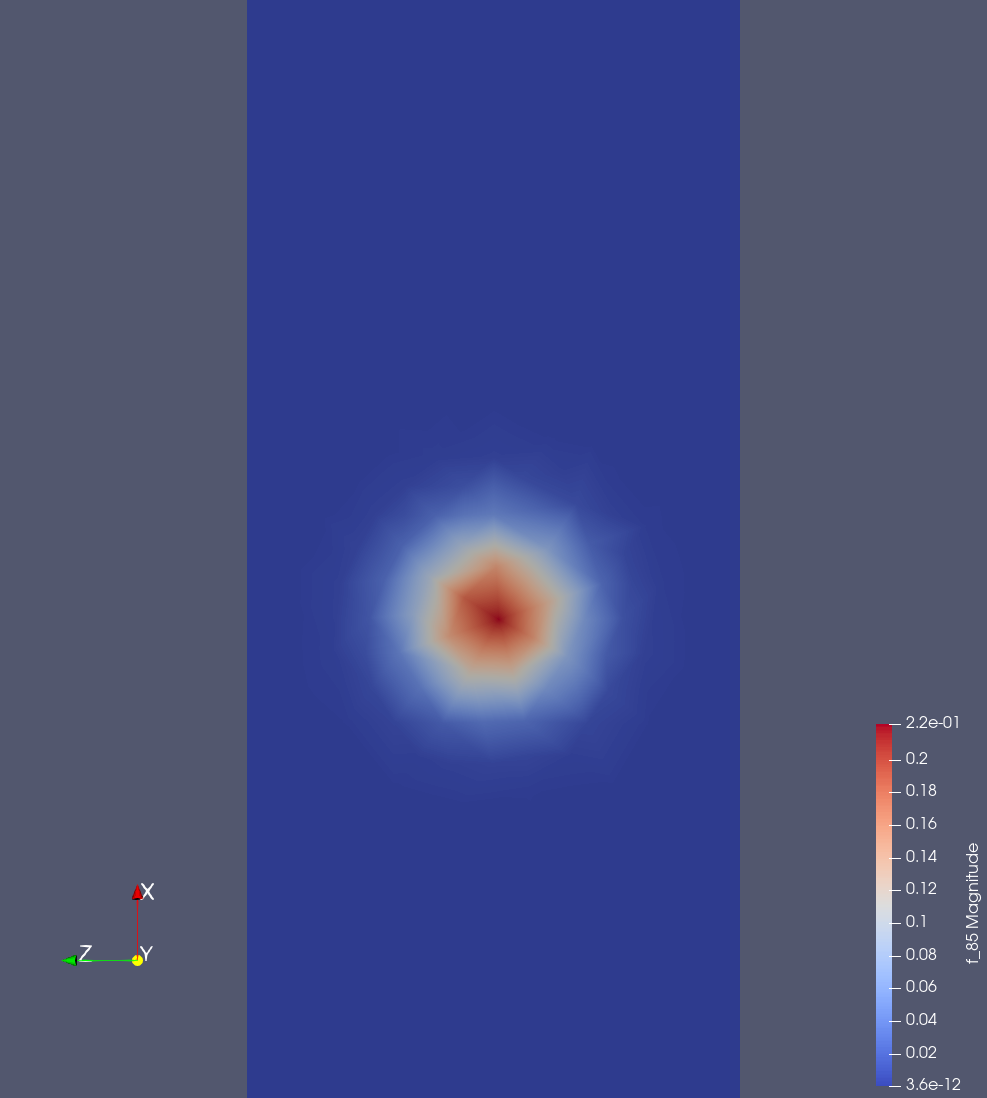
\includegraphics[width=0.49\textwidth]{./resources/fwd_bot}
    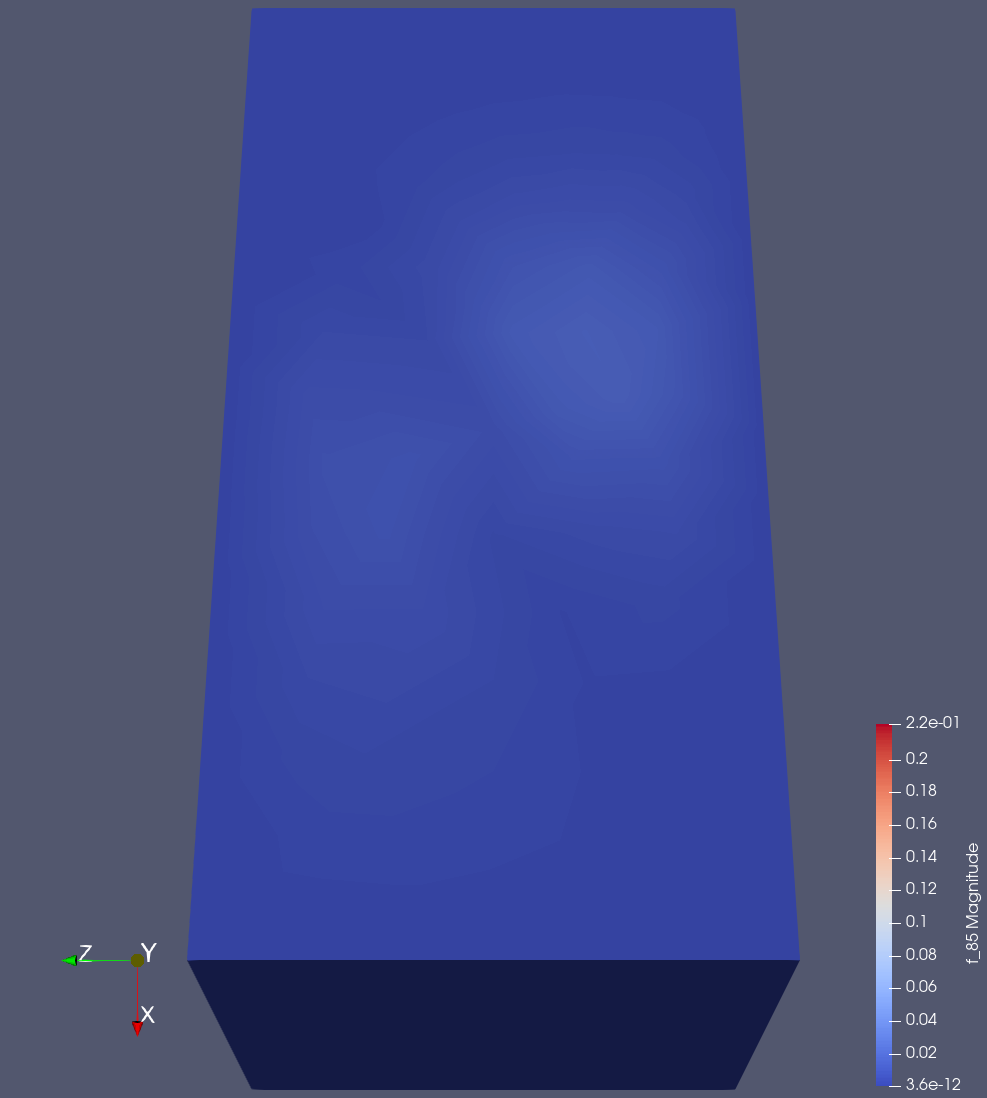
\includegraphics[width=0.49\textwidth]{./resources/fwd_top}
  \end{figure}
\end{frame}
\begin{frame}
  \frametitle{Forward Solution}
  \begin{figure}
    \centering
    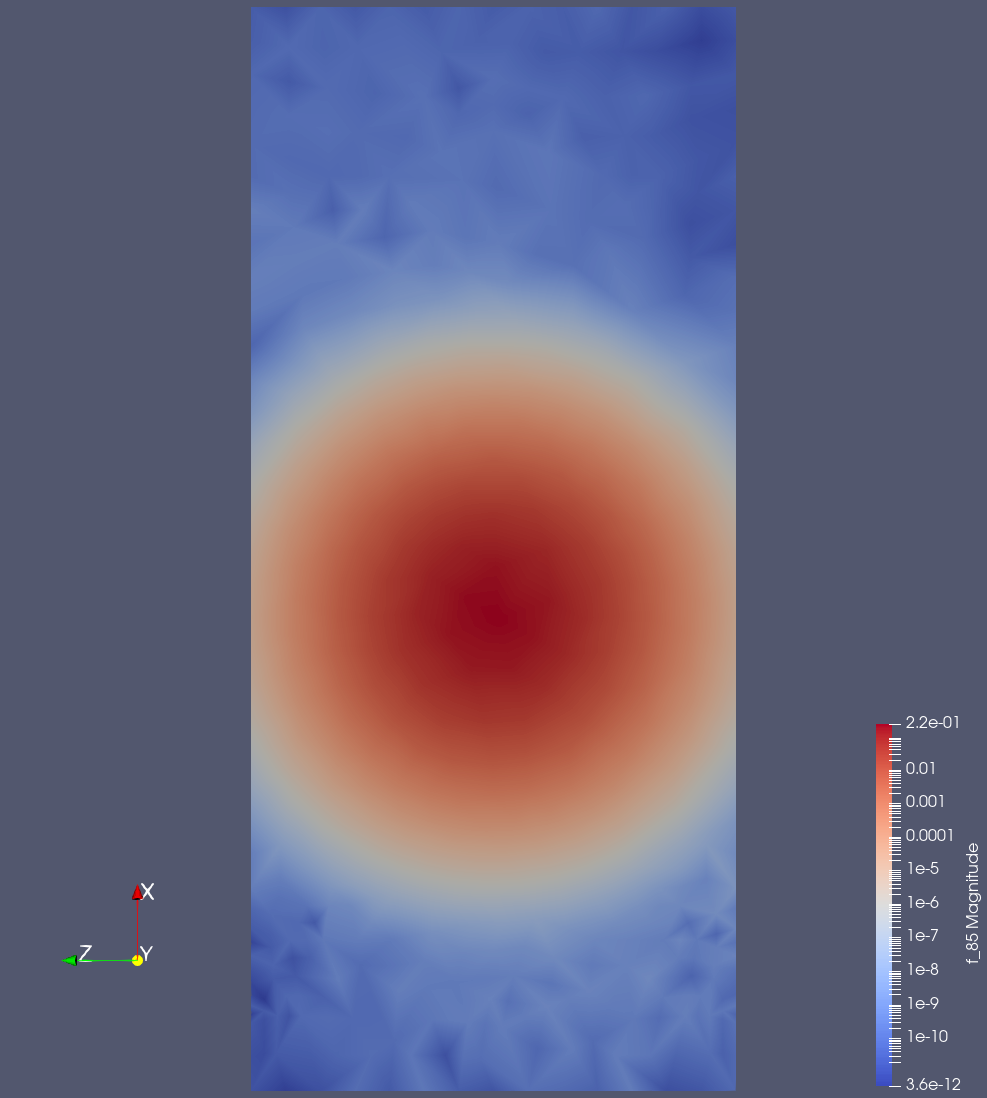
\includegraphics[width=0.49\textwidth]{./resources/fwd_bot_log}
    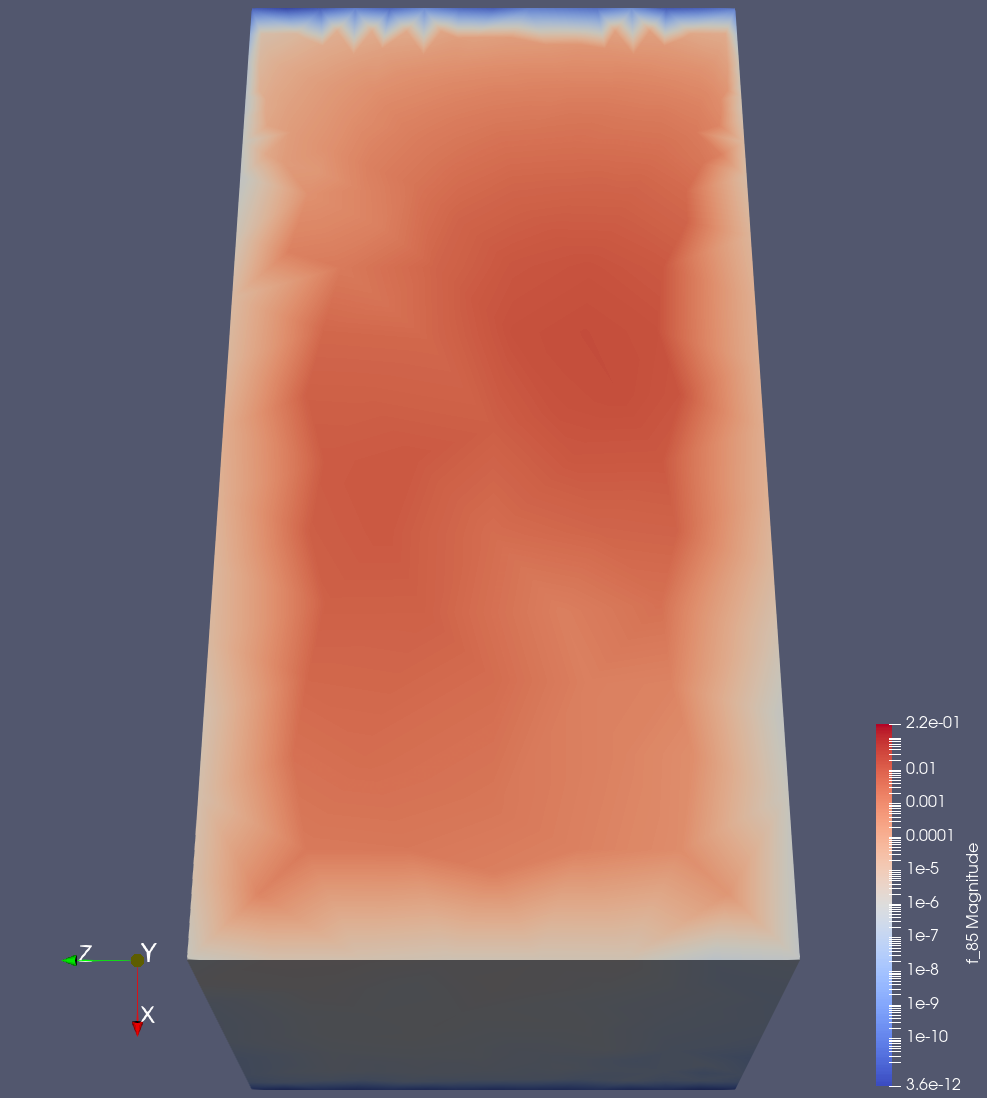
\includegraphics[width=0.49\textwidth]{./resources/fwd_top_log}
  \end{figure}
\end{frame}

\begin{frame}
  \frametitle{Weak Formulation}
  Define:
  \[
    \vec{V} \coloneqq
    \{ 
      \vec{u} \in H^1(\Omega)^3 
      : \vec{u} \vdot \vec{n} = 0 \text{ on } \Gamma_b
    \}
  \]
  Then the weak formulation of the forward model is given by:
  \begin{multline}
    \int_{\Gamma_s} \beta^{-1} (\vec{u} - \vec{h}) \vdot \vec{v} \dd{s}
    + \int_{\Gamma_b} \delta^{-1} (\mat{T} \vec{u} - \vec{m}) \vdot \vec{v}
    \dd{s} \\
    + \int_\Omega \vec{\e}(\vec{u}) : \mathbb{C}[\vec{\e}(\vec{v})] \dd{\vec{x}}
    = 0,
    \quad \forall v \in \vec{V}
  \end{multline}
\end{frame}

%%%%%%%%%%%%%%%%%%%%%%%%%%%%%%%%%%%%%%%%%%%%%%%%%%%%%%%%%%%%%%%%%%%%%%%%%%%%%%
%%% Bayesian Inversion Setting
%%%%%%%%%%%%%%%%%%%%%%%%%%%%%%%%%%%%%%%%%%%%%%%%%%%%%%%%%%%%%%%%%%%%%%%%%%%%%%%
\section{Infinite-Dimensional Inverse Problem Setting}
\begin{frame}
  \frametitle{The Deterministic Inverse Problem}
  To reconstruct the fault displacement we construct the PDE-constrained
  optimization problem:
  \[
    \mc{J}(\vec{m})
    = \frac{1}{2} \| \mc{B}\vec{u}(\vec{m}) - \obs \|^2
    + \frac{1}{2} \| \mc{A}\vec{m} \|^2
  \]
  where $\vec{u}$ is given by the solution of the linear elasticity equation.
  \begin{itemize}
    \item $\vec{u}(\vec{m})$ is given by the forward model.
    \item $\mc{B}: (L^2(\Omega))^3 \to \R^N$ is an observation operator.
    \item $\obs \in \R^N$ where $N$ is the number of data points.
  \end{itemize}
  \pause
  If we let $\mc{S}$ be the forward model operator, i.e. $\vec{u} = \mc{S}
  \vec{m}$, and let\footnote{%
    In literature, called the {\em parameter-to-observable operator}.
  } $\mc{F} = \mc{B} \mc{S}$, then:
  \[
    \mc{J}(\vec{m})
    = \frac{1}{2} \| \mc{F}\vec{m} - \obs \|^2
    + \frac{1}{2} \| \mc{A}\vec{m} \|^2
  \]
\end{frame}

\begin{frame}
  \frametitle{Bayesian Inversion in Finite Dimensions}
  \begin{theorem}[Bayes Theorem in Finite Dimensions]
    \[
      \pi_{\rm post}(\vb{m} | \mathbf{u}^{\rm obs})
      \propto
      \pi_{\rm like}(\mathbf{u}^{\rm obs} | \vb{m})
      \pi_{\rm prior}(\vb{m})
    \]
  \end{theorem}
  \begin{itemize}
    \item Gaussian Prior $\vb{m} \sim \mc{N}(\vb{m}_{\rm pr}, \mat{\Gamma}_{\rm pr})$.
    \item Additive Gaussian noise
      \[
        \obs = \mat{F} \vb{m} + \vb*{\eta},
        \quad \vb*{\eta} \sim \mc{N}(\vb{0}, \mat{\Gamma}_{\rm noise})
      \]
    \item Posterior is therefore Gaussian with:
      \[
        \vb{m} | \mathbf{u}^{\rm obs} 
        \sim \mc{N}(\vb{m}_{\rm post} , \vb{\Gamma}_{\rm post})
      \]
      where:
      \begin{align*}
        \vb{m}_{\rm post}
        &=
        \vb{\Gamma}_{\rm post}
        \left(
          \mat{F}^\T \vb{\Gamma}_{\rm noise}^{-1} \mathbf{u}^{\rm obs}
          + \vb{\Gamma}_{\rm pr}^{-1} \vb{m}_{\rm pr}
        \right) \\
        \vb{\Gamma}_{\rm post}
        &=
        \left(
          \mat{F}^\T \vb{\Gamma}_{\rm noise}^{-1} \mat{F}
          + \vb{\Gamma}_{\rm pr}^{-1}
        \right)^{-1} \\
      \end{align*}
  \end{itemize}
  Corresponds to
  \(
    \mc{J}(\vb{m})
    = \frac{1}{2} \| \mc{F}\vb{m} - \obs \|_{\vb{\Gamma}_{\rm noise}^{-1}}^2
    + \frac{1}{2} \| \vb{m} - \vb{m}_{\rm pr}\|_{\vb{\Gamma}_{\rm pr}^{-1}}^2
  \).
\end{frame}
\begin{frame}
  \frametitle{Bayesian Inversion in Infinite Dimensions}
  \begin{theorem}[Bayes Theorem in Infinite Dimensions]
    \[
      \dv{\mu^{\obs}_{\rm post}}{\mu_{\rm pr}}
      \propto
      \pi_{\rm like}(\obs | \vec{m})
    \]
  \end{theorem}
  \begin{itemize}
    \item Gaussian Prior $\vec{m} \sim \mc{N}(\vec{m}_{\rm pr}, \mc{C}_0)$.
    \item Additive Gaussian noise
      \[
        \obs = \mc{F} \vec{m} + \vb*{\eta},
        \quad \vb*{\eta} \sim \mc{N}(\vb{0}, \mat{\Gamma}_{\rm noise})
      \]
    \item The pair $(\vec{m}, \obs)$ is jointly Gaussian with:
      \[
        \mu^{\obs}_{\rm post}
        =
        \mc{N}(\vec{m}_{\rm post} , \mc{C}_{\rm post})
      \]
      where:
      \begin{align*}
        \vec{m}_{\rm post}
        &=
        \mc{C}_{\rm post}
        \left(
          \mc{F}^* \vb{\Gamma}_{\rm noise}^{-1} \obs
          + \mc{C}_{\rm pr}^{-1} \vec{m}_{\rm pr}
        \right) \\
        \mc{C}_{\rm post}
        &=
        \left(
          \mc{F}^* \vb{\Gamma}_{\rm noise}^{-1} \mc{F}
          + \mc{C}_{\rm pr}^{-1}
        \right)^{-1} \\
      \end{align*}
  \end{itemize} \vspace{-1em}
  Corresponds to
  \(
    \mc{J}(\vec{m})
    = \frac{1}{2} \| \mc{F}\vec{m} - \obs \|_{\vb{\Gamma}_{\rm noise}^{-1}}^2
    + \frac{1}{2} \| \mc{C}^{-1/2}(\vec{m}-\vec{m}_{\rm pr}) \|^2
  \).
\end{frame}

\begin{frame}
  \frametitle{Returning to Fault Inversion}
  \textbf{Slight Wrinkle:} Our parameter-to-observable map is affine.
  \pause
  \begin{block}{}
    We want to minimize
    \[
      \mc{J}(\vec{m})
      = \frac{1}{2} \| \mc{B}\vec{u} - \obs \|_{\vb{\Gamma}_{\rm noise}^{-1}}^2
      + \frac{1}{2} \| \mc{C}^{-1/2}(\vec{m}-\vec{m}_{\rm pr}) \|^2
    \]
  \end{block}
  \pause
  Define:
  \begin{align*}
    \mc{L}(\vec{m}, \vec{u}, \vec{v})
    &= \frac{1}{2} \| \mc{B}\vec{u} - \obs \|_{\vb{\Gamma}_{\rm noise}^{-1}}^2
    + \frac{1}{2} \| \mc{C}^{-1/2}(\vec{m}-\vec{m}_{\rm pr}) \|^2 
    + \int_{\Gamma_s} \beta^{-1} (\vec{u} - \vec{h}) \vdot \vec{v} \dd{s} \\
    &+ \int_{\Gamma_b} \delta^{-1} (\mat{T} \vec{u} - \vec{m}) \vdot \vec{v}
    \dd{s} 
    + \int_\Omega \vec{\e}(\vec{u}) : \mathbb{C}[\vec{\e}(\vec{v})] \dd{\vec{x}}
  \end{align*}
  \textbf{Procedure:} Obtain $\vec{m}$ by enforcing $\mc{L}_\vec{m}
  = \mc{L}_\vec{u} = \mc{L}_\vec{v} = 0$.
\end{frame}

%%%%%%%%%%%%%%%%%%%%%%%%%%%%%%%%%%%%%%%%%%%%%%%%%%%%%%%%%%%%%%%%%%%%%%%%%%%%%%%
%%% Numerical Discretization and Considerations
%%%%%%%%%%%%%%%%%%%%%%%%%%%%%%%%%%%%%%%%%%%%%%%%%%%%%%%%%%%%%%%%%%%%%%%%%%%%%%%
\section{Numerical Discretization and Considerations}
\begin{frame}
  \frametitle{FEM Discretization}
  \begin{itemize}
    \item Consider finite element space $\mc{V}_h = {\rm Span}(\phi_1, \dots,
      \phi_n)$.
    \item $\phi_k$: Lagrange basis functions. 
    \item For $\vb{f} \in \mc{V}_h$:
      \[
        \vb{f} = \sum_{k=1}^n f_k \phi_k
      \]
    In particular, construct $\vb{u}, \vb{v}, \vb{m}, \vb{m}_{\rm pr},
      \vb{h} \in \mc{V}_h$ from $\vec{u}, \vec{v}, \vec{m}, \vec{m}_{\rm pr}$
      and $\vec{h}$.
    \item Finite dimensional Hilbert space 
      \[
        (\mc{V}_h, \inp{\cdot}{\cdot}_{L^2})
        \cong 
        (\R^n, \inp{\cdot}{\cdot}_M),
        \qquad \inp{\vb{u}}{\vb{v}} = \vb{u}^\T \mat{M} \vb{v}
      \]
    \item From the Lagrangian we find
      \[
        \begin{bmatrix}
          \mat{C}_{\rm pr}^{-1} & & -\mat{C}^* \\
          & \mat{B}^* \vb{\Gamma}_{\rm noise}^{-1} \mat{B} & \mat{A}^* \\
          -\mat{C} & \mat{A} & 
        \end{bmatrix}
        \begin{bmatrix} \vb{m} \\ \vb{u} \\ \vb{v} \end{bmatrix}
        = \begin{bmatrix}
          \mat{C}_{\rm pr}^{-1} \vb{m}_0 \\ 
          \mat{B}^* \vb{\Gamma}_{\rm noise}^{-1} \obs \\
          \mat{D} \vb{h}
        \end{bmatrix}
      \]
      where $\mat{A} \vb{u} = \mat{C} \vb{m} + \mat{D} \vb{h}$ is the discretized
      weak form.
  \end{itemize}
\end{frame}
\begin{frame}
  \frametitle{Reduced Linear System}
  \begin{block}{Parameter-to-Observable Map}
    From the discretized weak form we can define:
    \[
      \mat{A}\vb{u} = \mat{C} \vb{m} + \mat{D} \vb{h}
      \implies
      \mc{F}(\vb{m}) = \mat{B} \mat{A}^{-1} \left[
        \mat{C} \vb{m} + \mat{D} \vb{h}
      \right]
      = \mc{G} \vb{m} + \vb{g}
    \]
  \end{block}
  \pause
  With this:
  \[
    \begin{bmatrix}
      \mat{C}_{\rm pr}^{-1} & & -\mat{C}^* \\
       & \mat{B}^* \vb{\Gamma}_{\rm noise}^{-1} \mat{B} & \mat{A}^* \\
      -\mat{C} & \mat{A} & 
    \end{bmatrix}
    \begin{bmatrix} \vb{m} \\ \vb{u} \\ \vb{v} \end{bmatrix}
    = \begin{bmatrix}
      \mat{C}_{\rm pr}^{-1} \vb{m}_0 \\ 
      \mat{B}^* \vb{\Gamma}_{\rm noise}^{-1} \obs \\
      \mat{D} \vb{h}
    \end{bmatrix}
  \]
  can be reduced to
  \[
    \left(
      \mat{C}_{\rm pr}^{-1} + \mc{G}^* \vb{\Gamma}_{\rm noise}^{-1} \mc{G}
    \right)\vb{m}
    = \mc{G}^* \vb{\Gamma}_{\rm noise}^{-1} \left( \vb{g} + \obs \right)
    + \mat{C}_{\rm pr}^{-1} \vb{m}_0
  \]
\end{frame}

\begin{frame}
  \frametitle{Tractability of Computation}
  \[
    \underbrace{\left[
        \mat{C}_{\rm pr}^{-1} + \mc{G}^* \vb{\Gamma}_{\rm noise}^{-1} \mc{G}
    \right]}_{\mat{C}_{\rm post}^{-1}}
    \vb{m}_{\rm post}
    =
    \left[
      \mc{G}^* \vb{\Gamma}_{\rm noise}^{-1} \left( \vb{g} + \obs \right)
      + \mat{C}_{\rm pr}^{-1} \vb{m}_0
    \right]
  \]
  How do we make this computation tractable?
  \pause
  \begin{itemize}
    \item Exploit the dimensionality reduction in the parameter space
    \item Use symmetry aware solvers
    \item Leverage sparsity of 
      \begin{itemize}
        \item matrices induced by differential operators
        \item observations
      \end{itemize}
  \end{itemize}
\end{frame}

\begin{frame}
  \frametitle{Parameter space dimensionality reduction}
\end{frame}

\begin{frame}
  \frametitle{Symmetry: Adjoints want to kill you}
\end{frame}

\begin{frame}
  \frametitle{Sparsity: Matrices induced by differential operators}
\end{frame}

\begin{frame}
  \frametitle{Sparsity: Observations}
\end{frame}

%%%%%%%%%%%%%%%%%%%%%%%%%%%%%%%%%%%%%%%%%%%%%%%%%%%%%%%%%%%%%%%%%%%%%%%%%%%%%%%
%%% Results
%%%%%%%%%%%%%%%%%%%%%%%%%%%%%%%%%%%%%%%%%%%%%%%%%%%%%%%%%%%%%%%%%%%%%%%%%%%%%%%
\section{Results}

%%%%%%%%%%%%%%%%%%%%%%%%%%%%%%%%%%%%%%%%%%%%%%%%%%%%%%%%%%%%%%%%%%%%%%%%%%%%%%%
%%% Discussion and Future Work
%%%%%%%%%%%%%%%%%%%%%%%%%%%%%%%%%%%%%%%%%%%%%%%%%%%%%%%%%%%%%%%%%%%%%%%%%%%%%%%
\section{Discussion and Future Work}


%%%%%%%%%%%%%%%%%%%%%%%%%%%%%%%%%%%%%%%%%%%%%%%%%%%%%%%%%%%%%%%%%%%%%%%%%%%%%%%
%%% References
%%%%%%%%%%%%%%%%%%%%%%%%%%%%%%%%%%%%%%%%%%%%%%%%%%%%%%%%%%%%%%%%%%%%%%%%%%%%%%%
\section{References}
\begin{frame}[allowframebreaks]
  \frametitle{References}
  \printbibliography
\end{frame}

\end{document}
